\subsection{Report Validation}
\begin{figure}[H]
  \centering
  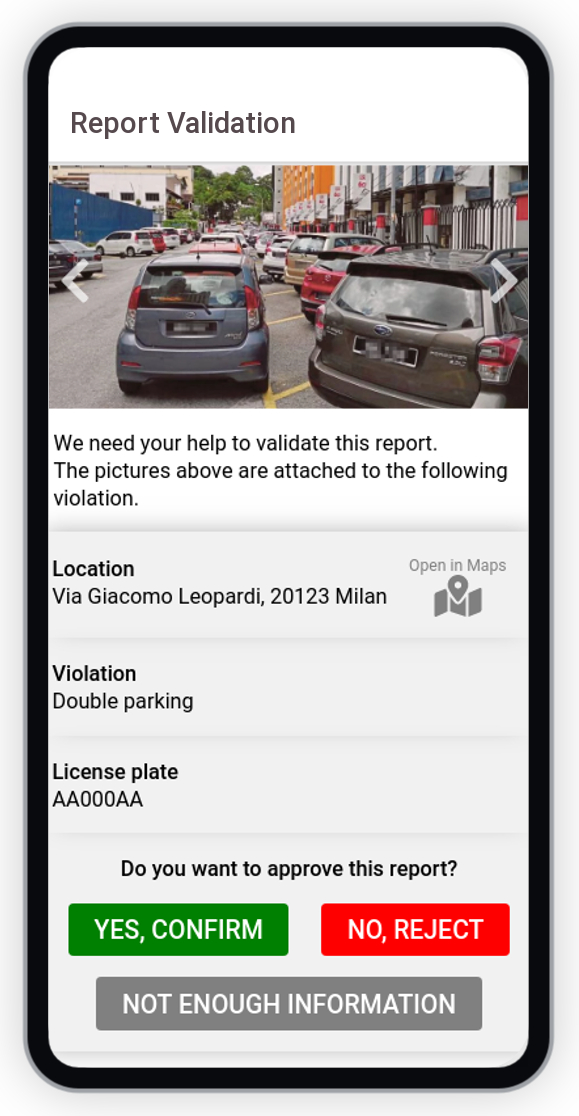
\includegraphics[origin=c,width=\textwidth,height=.70\textheight,keepaspectratio]{DD_Images/UserInterface/Validation.jpg}
  \caption{\textit{Report Validation}}
\end{figure}

Reports are validated by the community, so every time a new violation is submitted to SafeStreets some users will be notified and will see this screen.
The report is anonymous, so the users that validate it don't see who sent it, but only the relevant details about the notified infraction. 
The user is therefore asked to click one of the three buttons to either validate, reject or ignore the report.